\setchapterpreamble[u]{\margintoc}
\chapter{Creativity and Decision Making with Deep Learning Models}
\labch{intro}

\textit{"AI Policy}

\textit{I expect you to use AI (ChatGPT and image generation tools, at a minimum), in this class. In fact, some assignments will require it. Learning to use AI is an emerging skill, and I provide tutorials in Canvas about how to use them. I am happy to meet and help with these tools during office hours or after class}

\textit{Beware of the limits of ChatGPT:}

\begin{itemize}
	\item\textit{If you provide minimum effort prompts, you will get low quality results. You will need to refine you prompts to get good outcomes. This will take work.}
	\item\textit{Don't trust anything it says. If it gives you a number or a fact, assume it is wrong unless you either know the answer or can check in with another source. You will be responsible for any errors or omissions provided by the tool. It works best for topics you understand.}
	\item\textit{AI is a tool, but one that you need to acknowledge using. Please include a paragraph at the end of any assignment that uses AI explaining what you used the AI for and what prompts you used to get the results. Failure to do so is in violation of academic honesty policies}
	\item\textit{Be thoughtful about when this tool is useful. Don't use it if it isn't appropriate for the case or circumstance."}
\end{itemize}

\textit{Dr. Ethan Mollick, 2023 - Syllabus for class at The Wharton School at the University of Pennsylvania}


\section{Theories of Creativity}

Machine learning models use data (from the past) to discover rules and make classifications. Because of the way they are constructed these classifications, suggestions, artworks are by definition derivative or "having parts that originate from another source". I won't get into a philosophical discussion on what the nature of creativity is, but it's worth considering how using deep learning AI models biases us towards the past, but also could give us insights from other domains. 

\begin{marginfigure}[-5.5cm]
        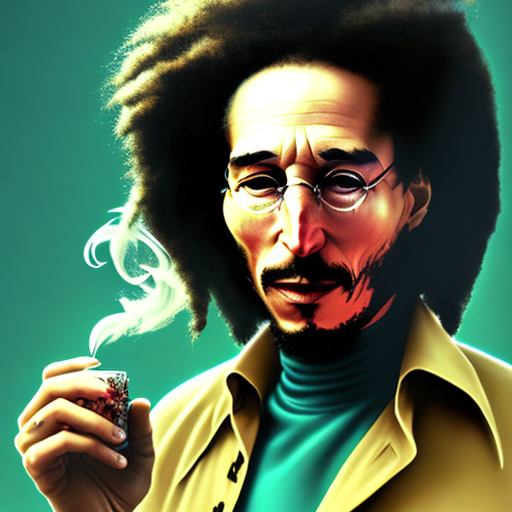
\includegraphics{jobsweed}
        \caption{"mdjrny-v4 Steve Jobs Smoking weed with Bob Marley 8k" made with Mann-E. It's 100\% derivative, but it's art too (I guess).}
        \labfig{jobsweed}
\end{marginfigure}

It can be argued that creativity is simply the combination of existing works. This is because many new ideas and innovations are often inspired by and built upon existing concepts. For example, a new form of music may be created by combining elements from different genres. Similarly, a new technology may be created by combining and improving upon existing technologies.

It can also be argued that creativity involves much more than just combining existing works. Creativity is not just about recombining existing ideas, but also about coming up with completely new and original concepts. This requires a unique perspective and a deep understanding of the subject matter, as well as the ability to think outside the box.  

AI models of speech, when heavily used, may slow down the evolution of language. AI art models may slow down "progress" in art, whatever that means. AI models of disease trained on data from 1980 may be irrelevant to today's diseases\sidenote{We'll discuss "concept drift" later, don't worry.}. That said these same models may give us interesting insights in new domains, models trained on beautiful paintings may be put to use in a new domain (like desiging beautiful interiors) and that model could give new insight to interior designers, models of the interaction of ants could be put to use in designing cities and so on and so forth. AI cuts many ways, it makes us faster but makes us more reliant on the past, models can be used across domains but should be used intentionally and transparently when possible. Each use opens up a new world of possibilites for users, and sometimes a new headache for intellectual property lawyers. We'll discuss all of these topics in this chapter.


\section{Creative Uses of Power Tools}

Power tools, even simple ones like a drill\sidenote{something like these \url{https://www.dewalt.com/products/power-tools/drills}} are complex machines that take human input and transform it using static rules. The pressure the user of a drill puts on the bit and the speed at which they pull the trigger all deterministically affect the output. Just because a tool is a deterministic machine doesn't mean it is unable to produce creatve works.

What is happening as we use generative tools like ChatGPT or image-to-textmodels is that the "creative act" has been relocated. The creative act is now the prompt you give the tool, the users input. And someone can still be good at using AI, just like someone can be good at using any piece of software.

Modern AI is a complex system of algorithms, data, and analytics that can be used to solve complex problems. AI systems can learn from data, identify patterns, and make predictions about the future. AI systems are typically used to automate and assist human decision making. AI systems are programmed with specific objectives and goals, and the user input decides the output. For example, an AI system could be programmed to solve a mathematical problem and the user input would determine the parameters of the problem and the output would be the solution.

A power drill is also a complex deterministic system. The user input is limited to the type of drill bit, the speed of the drill, and the direction of the drill. The output is determined by these inputs, as the drill will only drill in the direction and speed determined by the user. The user also has to choose the correct drill bit to ensure the drill can do the job correctly and safely.

\begin{marginfigure}[-5.5cm]
        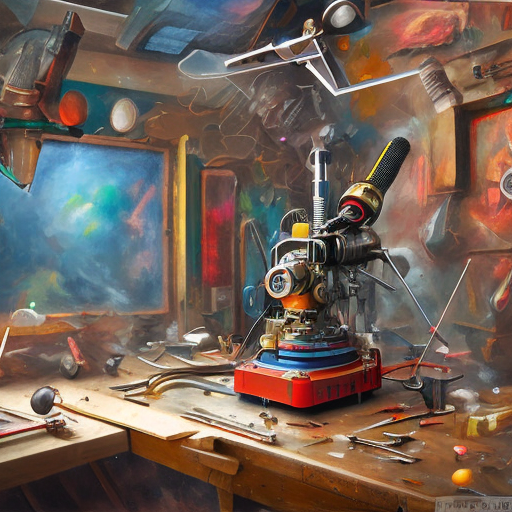
\includegraphics{drillart}
        \caption{"mdjrny-v4 a mikita drill being used in an artist's studio to make a colorful artwork 8k" made with Mann-E}
        \labfig{drillart}
\end{marginfigure}

Overall, both modern AI and a power drill are complex but ultimately deterministic systems. The user input, however limited it may be, ultimately controls the output of the system. Both systems require a user to understand how to use them and to make the correct input to get the desired output.

\section{Garbage In, Garbage Out}

The "Power Tool" of AI is a deterministic \sidenote{and static or unchanging} system and the rules of that system are determined by the data that the model is shown. If a model is trained on shitty\sidenote{scientific term here} data, it will produce shitty results. End of book...

... maybe not. It's worth thinking about this for a moment. It is often said that modern AI can "generalize and make informed inferences given new data". If deep learning models are really just a big regression, these models will always come up with an answer, but if the world changes, these models will still be projecting complicated averages of their past data into the future.\sidenote{I'm going to talk about concept drift in a few paragraphs, I promise} 

So, let's separate AI's decision making into two extremes; \textit{Creative Decision Making} and \textit{Critical Decision Making}. The stakes are very low in a world of \textit{Creative Decision Making} and who gives a shit if the AI is all a regression, and it just mushes together the limited data that it's seen. In a creative context you can also ask an AI interesting questions, so long as you don't soley rely on it's output without checking the facts first\sidenote{see the syllabus note at the beginning of this chapter}. Even if "Garbage In, Garbage Out" holds, garbage can still be helpful for a creative process. 

Note that this book is called "Full-Self Driving, Skynet..", a self-driving car and a nuclear-bomb-equipped all-seeing AI are clearly not engaging in any \textit{Creative Decision Making}. I'll spend lot's of time diving into this but this distintion is super important. 

\textbf{Modern AI, particularly deep learning models, will never be reliable enough to make critical decisions by themselves.} These models will transform the nature of work and jobs and do a lot of things, but because of the nature of how these models are created, they should \textbf{never} be relied on to make critical decisions by themselves. If you think this point is obvoius and pedantic, just stop reading I guess. But the general public seems to be confused about this point, so I'm going to discuss it in depth for many chapters. I'll say here that there are also many ways to reign in deep learning models and allow them to participate in critical decision making without having the final say, most of them involve humans getting a vote, others involve putting the deep learning model 'on rails' and either programming explicit rules via GOFAI or by physical systems that limit the deep learning model's decision making capacity\sidenote{Imagine a self-driving train that can only go so fast, and is mechanically setup to brake at certian intervals or locations, plus has a human watcher who can take over if things get weird. I like this train.}.


\section{Garbage In, New Perspective Out?}

For creative tasks, it generally doesn't matter that a deep learning model is unscientific or trained on a lopsided dataset. An informed user of AI knows this and can account for that in their decision making, especially when engaging in creative decision making. The situation becomes problematic once we allow deep learning models to engage in critical decision making by themselves. Allow me to enumerate a few examples:

\begin{enumerate}
    \item \textbf{A text generation model trained on Shakespeare's plays} This could be used to spruce up dialoge for a screenplay, write a book, or write a fancy-sounding email. It should be obvious to the user what it is doing, and this would probably delight users and not cause many problems.
    \item \textbf{A in image classifier for a dating app, trained on images of famous couples} Someone wants to start their own dating app, but they don't have any of their own data. So they base their "compatability score" off of photos of potential couple and classify them as either "looking like a celebrity couple, and therefore compatable" or "not looking like a celebrity couple, and therefore incompatable". This model sounds funny and interesting, but could certainly change lives. I still would say this is a creative use of a model, and probably fine. 
    \item \textbf{A threat classifier traned on images of war} Wars might change from place to place, if the model was trained in the middle east it might not be as useful in Ukraine, but maybe it could be helpful to augment a security guard looking over thousands of cameras at Grand Central Station. It is not clear to me whether classifying threats falls under creative or critical decision making. Is this a useful classifier for an understaffed security unit, or a bias-reinforcing tool for police abuse? I'm not sure, but I'm sure this model is out there already.\sidenote{if you would like a deeper discussion of ethics please read Reid Blackman's "Ethical Machines"\cite{Blackman2022Jul}, he is pretty good for a Philosophy PhD.}
    \item \textbf{A text generation model claiming to be Artificial General Intelligence}\sidenote{Let's say something like ChatGPT} A model using deep learning techniques, and trained on the entire internet, but claiming to have general purpose answers to everything\sidenote{ChatGPT does not make these claims}. This could absolutely be used for creative endeavors and generate new perspectives but if it is given critical tasks and relied on to "tell the truth", this will probably disappoint. Creating the model isn't a problem in itself, but how it is used or misused might cause a problem.\sidenote{What problems, you ask? Well, give me a few chapters.}
    \item \textbf{A fully self-driving car, one without a steering wheel} The car was trained on millions of miles of road-trials, and maybe a sophisticated simulation environment where it drove trillions of virtual miles.\sidenote{Let's assume the model is only updated once per month here, I'll talk about this in more depth soon.} This model is not giving you a new perspective or funny perspective on driving because all of the training happened in the past. So, as soon as the self-driving model is released, it becomes stale. Any significant changes in the envoronment might cause it to behave strangely and dangerously.
\end{enumerate}

I will talk about many of these models in depth in the coming chapters, but it's worth sticking them into your brain now. The models themselves are not good or bad, they are a product of the data they were shown, how they are used and the decision making ability they are given makes them either fun and amazing, or dangerous and foolish.

\begin{marginfigure}[-5.5cm]
        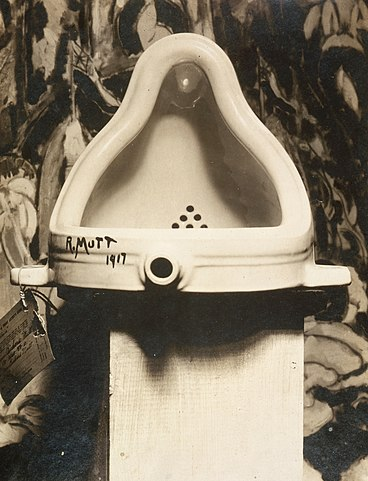
\includegraphics{duchamp}
        \caption{Marcel Duchamp's "Fountain". A urinal that blew peoples minds \url{https://www.tate.org.uk/art/artworks/duchamp-fountain-t07573}.}
        \labfig{duchamp}
\end{marginfigure}

One last note before I shut up about creativity, generative models will come up with amazing (but derivative) works of art, But, they will never "change the game". A model of sculpture trained on past sculptures in 1917 will never come up with Marcel Duchamp's "Fountain". There is a term that machine learning engineers use for this, when the rules of the game are changed, it's called "Concept Drift".

\section{Concept Drift and the end of usefulness}

When the meaning of truth changes.

\section{The Impossibility of Fairness}

Representation, "fixing the training set" \sidecite{Christian2020}, or the Impossibility of Fairness from a model.

\section{What Are We Prediciting Again?}

are you predicting the right thing? Are you really predicting how valuable the company is or just whether it'll be the next meme stock?

\section{Humans Love Computers}

Working together seems like a good idea, but how. Talk about 2 percent model control and model uptake. 

Also talk about Kasparov's tournament and Thinking for yourself in the age of AI. \sidecite{mansharamani2020}

Oneil\cite{Oneil2017}
Perez\cite{Perez2019}
Blackman\cite{Blackman2022Jul}
Christian\cite{Christian2020}

\section{Key Takeaways}

\begin{itemize}
    \item \textbf{Deep learning models are fundamentally large unscientific regressions} they are trained to create a function that maps input data to output data.
    \item \textbf{Deep learning models are chaotic systems containing millions of interacting parameters} they are not designed to be explained or created in a way that their weights can be used for scientific analysis. They find reasonable answers and don't care how they get there. Multicolinearity (understanding the relationship of an input and output) and feature importance (understanding which inputs are most important) are only understandable with a high level of statistical error.
    \item \textbf{Small changes in inputs of a deep learning model may dramatically change the outputs} deep learning models are complex deterministic systems that can exhibit chaotic behavior. Their inner workings are functionally unknowable and practically impossible to test.
    \item \textbf{Deep learning models can have impressive and useful outputs, but the creators of models should be encouraged to highlight their failures and limitations.} Machine learning engineers might be more keen to highlight failures and limitations if they are encouraged to do so by their users, managers and investors.
\end{itemize}

